\documentclass[border=6pt]{standalone}
\usepackage[utf8]{inputenc}\usepackage[T1]{fontenc}\usepackage{lmodern}\usepackage[english]{babel}
\usepackage{amsmath,amssymb}\usepackage{tikz}\usetikzlibrary{arrows.meta,positioning,calc,decorations.pathreplacing}
\begin{document}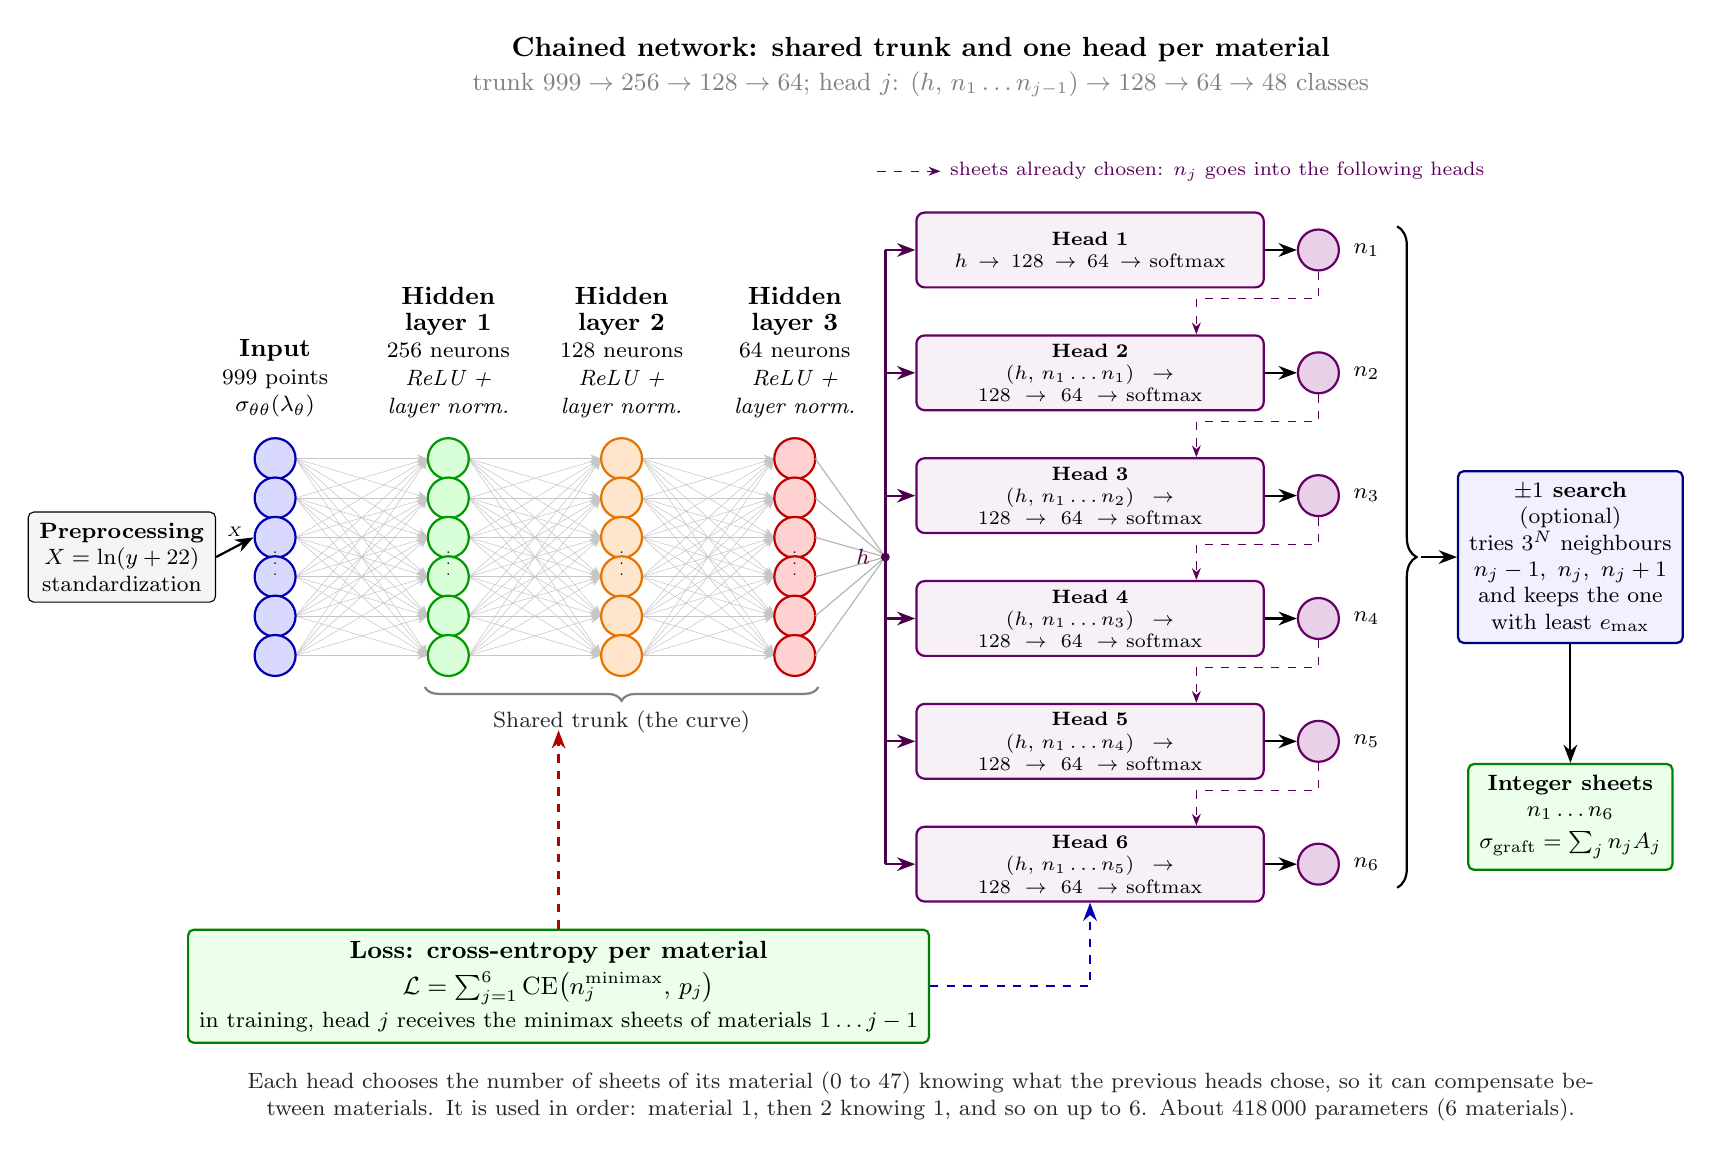
\begin{tikzpicture}[font=\small, n/.style={circle,draw,thick,minimum size=5.2mm,inner sep=0pt},
 box/.style={draw,rounded corners=2pt,fill=gray!8,align=center,inner sep=4pt,font=\footnotesize},
 hd/.style={draw=violet!80!black,thick,rounded corners=3pt,fill=violet!6,align=center,inner sep=3pt,font=\scriptsize,text width=4.2cm,minimum height=0.95cm}]
\node[font=\bfseries\normalsize] at (8.2,6.45) {Chained network: shared trunk and one head per material};
\node[gray] at (8.2,6.0) {trunk $999\to256\to128\to64$; head $j$: $(h,\,n_1\ldots n_{j-1})\to128\to64\to48$ classes};
\draw[-{Stealth[length=1.4mm]},gray!45,very thin] (0.26,1.25)--(1.94,1.25);
\draw[-{Stealth[length=1.4mm]},gray!45,very thin] (0.26,1.25)--(1.94,0.75);
\draw[-{Stealth[length=1.4mm]},gray!45,very thin] (0.26,1.25)--(1.94,0.25);
\draw[-{Stealth[length=1.4mm]},gray!45,very thin] (0.26,1.25)--(1.94,-0.25);
\draw[-{Stealth[length=1.4mm]},gray!45,very thin] (0.26,1.25)--(1.94,-0.75);
\draw[-{Stealth[length=1.4mm]},gray!45,very thin] (0.26,1.25)--(1.94,-1.25);
\draw[-{Stealth[length=1.4mm]},gray!45,very thin] (0.26,0.75)--(1.94,1.25);
\draw[-{Stealth[length=1.4mm]},gray!45,very thin] (0.26,0.75)--(1.94,0.75);
\draw[-{Stealth[length=1.4mm]},gray!45,very thin] (0.26,0.75)--(1.94,0.25);
\draw[-{Stealth[length=1.4mm]},gray!45,very thin] (0.26,0.75)--(1.94,-0.25);
\draw[-{Stealth[length=1.4mm]},gray!45,very thin] (0.26,0.75)--(1.94,-0.75);
\draw[-{Stealth[length=1.4mm]},gray!45,very thin] (0.26,0.75)--(1.94,-1.25);
\draw[-{Stealth[length=1.4mm]},gray!45,very thin] (0.26,0.25)--(1.94,1.25);
\draw[-{Stealth[length=1.4mm]},gray!45,very thin] (0.26,0.25)--(1.94,0.75);
\draw[-{Stealth[length=1.4mm]},gray!45,very thin] (0.26,0.25)--(1.94,0.25);
\draw[-{Stealth[length=1.4mm]},gray!45,very thin] (0.26,0.25)--(1.94,-0.25);
\draw[-{Stealth[length=1.4mm]},gray!45,very thin] (0.26,0.25)--(1.94,-0.75);
\draw[-{Stealth[length=1.4mm]},gray!45,very thin] (0.26,0.25)--(1.94,-1.25);
\draw[-{Stealth[length=1.4mm]},gray!45,very thin] (0.26,-0.25)--(1.94,1.25);
\draw[-{Stealth[length=1.4mm]},gray!45,very thin] (0.26,-0.25)--(1.94,0.75);
\draw[-{Stealth[length=1.4mm]},gray!45,very thin] (0.26,-0.25)--(1.94,0.25);
\draw[-{Stealth[length=1.4mm]},gray!45,very thin] (0.26,-0.25)--(1.94,-0.25);
\draw[-{Stealth[length=1.4mm]},gray!45,very thin] (0.26,-0.25)--(1.94,-0.75);
\draw[-{Stealth[length=1.4mm]},gray!45,very thin] (0.26,-0.25)--(1.94,-1.25);
\draw[-{Stealth[length=1.4mm]},gray!45,very thin] (0.26,-0.75)--(1.94,1.25);
\draw[-{Stealth[length=1.4mm]},gray!45,very thin] (0.26,-0.75)--(1.94,0.75);
\draw[-{Stealth[length=1.4mm]},gray!45,very thin] (0.26,-0.75)--(1.94,0.25);
\draw[-{Stealth[length=1.4mm]},gray!45,very thin] (0.26,-0.75)--(1.94,-0.25);
\draw[-{Stealth[length=1.4mm]},gray!45,very thin] (0.26,-0.75)--(1.94,-0.75);
\draw[-{Stealth[length=1.4mm]},gray!45,very thin] (0.26,-0.75)--(1.94,-1.25);
\draw[-{Stealth[length=1.4mm]},gray!45,very thin] (0.26,-1.25)--(1.94,1.25);
\draw[-{Stealth[length=1.4mm]},gray!45,very thin] (0.26,-1.25)--(1.94,0.75);
\draw[-{Stealth[length=1.4mm]},gray!45,very thin] (0.26,-1.25)--(1.94,0.25);
\draw[-{Stealth[length=1.4mm]},gray!45,very thin] (0.26,-1.25)--(1.94,-0.25);
\draw[-{Stealth[length=1.4mm]},gray!45,very thin] (0.26,-1.25)--(1.94,-0.75);
\draw[-{Stealth[length=1.4mm]},gray!45,very thin] (0.26,-1.25)--(1.94,-1.25);
\draw[-{Stealth[length=1.4mm]},gray!45,very thin] (2.46,1.25)--(4.14,1.25);
\draw[-{Stealth[length=1.4mm]},gray!45,very thin] (2.46,1.25)--(4.14,0.75);
\draw[-{Stealth[length=1.4mm]},gray!45,very thin] (2.46,1.25)--(4.14,0.25);
\draw[-{Stealth[length=1.4mm]},gray!45,very thin] (2.46,1.25)--(4.14,-0.25);
\draw[-{Stealth[length=1.4mm]},gray!45,very thin] (2.46,1.25)--(4.14,-0.75);
\draw[-{Stealth[length=1.4mm]},gray!45,very thin] (2.46,1.25)--(4.14,-1.25);
\draw[-{Stealth[length=1.4mm]},gray!45,very thin] (2.46,0.75)--(4.14,1.25);
\draw[-{Stealth[length=1.4mm]},gray!45,very thin] (2.46,0.75)--(4.14,0.75);
\draw[-{Stealth[length=1.4mm]},gray!45,very thin] (2.46,0.75)--(4.14,0.25);
\draw[-{Stealth[length=1.4mm]},gray!45,very thin] (2.46,0.75)--(4.14,-0.25);
\draw[-{Stealth[length=1.4mm]},gray!45,very thin] (2.46,0.75)--(4.14,-0.75);
\draw[-{Stealth[length=1.4mm]},gray!45,very thin] (2.46,0.75)--(4.14,-1.25);
\draw[-{Stealth[length=1.4mm]},gray!45,very thin] (2.46,0.25)--(4.14,1.25);
\draw[-{Stealth[length=1.4mm]},gray!45,very thin] (2.46,0.25)--(4.14,0.75);
\draw[-{Stealth[length=1.4mm]},gray!45,very thin] (2.46,0.25)--(4.14,0.25);
\draw[-{Stealth[length=1.4mm]},gray!45,very thin] (2.46,0.25)--(4.14,-0.25);
\draw[-{Stealth[length=1.4mm]},gray!45,very thin] (2.46,0.25)--(4.14,-0.75);
\draw[-{Stealth[length=1.4mm]},gray!45,very thin] (2.46,0.25)--(4.14,-1.25);
\draw[-{Stealth[length=1.4mm]},gray!45,very thin] (2.46,-0.25)--(4.14,1.25);
\draw[-{Stealth[length=1.4mm]},gray!45,very thin] (2.46,-0.25)--(4.14,0.75);
\draw[-{Stealth[length=1.4mm]},gray!45,very thin] (2.46,-0.25)--(4.14,0.25);
\draw[-{Stealth[length=1.4mm]},gray!45,very thin] (2.46,-0.25)--(4.14,-0.25);
\draw[-{Stealth[length=1.4mm]},gray!45,very thin] (2.46,-0.25)--(4.14,-0.75);
\draw[-{Stealth[length=1.4mm]},gray!45,very thin] (2.46,-0.25)--(4.14,-1.25);
\draw[-{Stealth[length=1.4mm]},gray!45,very thin] (2.46,-0.75)--(4.14,1.25);
\draw[-{Stealth[length=1.4mm]},gray!45,very thin] (2.46,-0.75)--(4.14,0.75);
\draw[-{Stealth[length=1.4mm]},gray!45,very thin] (2.46,-0.75)--(4.14,0.25);
\draw[-{Stealth[length=1.4mm]},gray!45,very thin] (2.46,-0.75)--(4.14,-0.25);
\draw[-{Stealth[length=1.4mm]},gray!45,very thin] (2.46,-0.75)--(4.14,-0.75);
\draw[-{Stealth[length=1.4mm]},gray!45,very thin] (2.46,-0.75)--(4.14,-1.25);
\draw[-{Stealth[length=1.4mm]},gray!45,very thin] (2.46,-1.25)--(4.14,1.25);
\draw[-{Stealth[length=1.4mm]},gray!45,very thin] (2.46,-1.25)--(4.14,0.75);
\draw[-{Stealth[length=1.4mm]},gray!45,very thin] (2.46,-1.25)--(4.14,0.25);
\draw[-{Stealth[length=1.4mm]},gray!45,very thin] (2.46,-1.25)--(4.14,-0.25);
\draw[-{Stealth[length=1.4mm]},gray!45,very thin] (2.46,-1.25)--(4.14,-0.75);
\draw[-{Stealth[length=1.4mm]},gray!45,very thin] (2.46,-1.25)--(4.14,-1.25);
\draw[-{Stealth[length=1.4mm]},gray!45,very thin] (4.66,1.25)--(6.34,1.25);
\draw[-{Stealth[length=1.4mm]},gray!45,very thin] (4.66,1.25)--(6.34,0.75);
\draw[-{Stealth[length=1.4mm]},gray!45,very thin] (4.66,1.25)--(6.34,0.25);
\draw[-{Stealth[length=1.4mm]},gray!45,very thin] (4.66,1.25)--(6.34,-0.25);
\draw[-{Stealth[length=1.4mm]},gray!45,very thin] (4.66,1.25)--(6.34,-0.75);
\draw[-{Stealth[length=1.4mm]},gray!45,very thin] (4.66,1.25)--(6.34,-1.25);
\draw[-{Stealth[length=1.4mm]},gray!45,very thin] (4.66,0.75)--(6.34,1.25);
\draw[-{Stealth[length=1.4mm]},gray!45,very thin] (4.66,0.75)--(6.34,0.75);
\draw[-{Stealth[length=1.4mm]},gray!45,very thin] (4.66,0.75)--(6.34,0.25);
\draw[-{Stealth[length=1.4mm]},gray!45,very thin] (4.66,0.75)--(6.34,-0.25);
\draw[-{Stealth[length=1.4mm]},gray!45,very thin] (4.66,0.75)--(6.34,-0.75);
\draw[-{Stealth[length=1.4mm]},gray!45,very thin] (4.66,0.75)--(6.34,-1.25);
\draw[-{Stealth[length=1.4mm]},gray!45,very thin] (4.66,0.25)--(6.34,1.25);
\draw[-{Stealth[length=1.4mm]},gray!45,very thin] (4.66,0.25)--(6.34,0.75);
\draw[-{Stealth[length=1.4mm]},gray!45,very thin] (4.66,0.25)--(6.34,0.25);
\draw[-{Stealth[length=1.4mm]},gray!45,very thin] (4.66,0.25)--(6.34,-0.25);
\draw[-{Stealth[length=1.4mm]},gray!45,very thin] (4.66,0.25)--(6.34,-0.75);
\draw[-{Stealth[length=1.4mm]},gray!45,very thin] (4.66,0.25)--(6.34,-1.25);
\draw[-{Stealth[length=1.4mm]},gray!45,very thin] (4.66,-0.25)--(6.34,1.25);
\draw[-{Stealth[length=1.4mm]},gray!45,very thin] (4.66,-0.25)--(6.34,0.75);
\draw[-{Stealth[length=1.4mm]},gray!45,very thin] (4.66,-0.25)--(6.34,0.25);
\draw[-{Stealth[length=1.4mm]},gray!45,very thin] (4.66,-0.25)--(6.34,-0.25);
\draw[-{Stealth[length=1.4mm]},gray!45,very thin] (4.66,-0.25)--(6.34,-0.75);
\draw[-{Stealth[length=1.4mm]},gray!45,very thin] (4.66,-0.25)--(6.34,-1.25);
\draw[-{Stealth[length=1.4mm]},gray!45,very thin] (4.66,-0.75)--(6.34,1.25);
\draw[-{Stealth[length=1.4mm]},gray!45,very thin] (4.66,-0.75)--(6.34,0.75);
\draw[-{Stealth[length=1.4mm]},gray!45,very thin] (4.66,-0.75)--(6.34,0.25);
\draw[-{Stealth[length=1.4mm]},gray!45,very thin] (4.66,-0.75)--(6.34,-0.25);
\draw[-{Stealth[length=1.4mm]},gray!45,very thin] (4.66,-0.75)--(6.34,-0.75);
\draw[-{Stealth[length=1.4mm]},gray!45,very thin] (4.66,-0.75)--(6.34,-1.25);
\draw[-{Stealth[length=1.4mm]},gray!45,very thin] (4.66,-1.25)--(6.34,1.25);
\draw[-{Stealth[length=1.4mm]},gray!45,very thin] (4.66,-1.25)--(6.34,0.75);
\draw[-{Stealth[length=1.4mm]},gray!45,very thin] (4.66,-1.25)--(6.34,0.25);
\draw[-{Stealth[length=1.4mm]},gray!45,very thin] (4.66,-1.25)--(6.34,-0.25);
\draw[-{Stealth[length=1.4mm]},gray!45,very thin] (4.66,-1.25)--(6.34,-0.75);
\draw[-{Stealth[length=1.4mm]},gray!45,very thin] (4.66,-1.25)--(6.34,-1.25);
\node[n,draw=blue!70!black,fill=blue!15] (n00) at (0.00,1.25) {};
\node[n,draw=blue!70!black,fill=blue!15] (n01) at (0.00,0.75) {};
\node[n,draw=blue!70!black,fill=blue!15] (n02) at (0.00,0.25) {};
\node[n,draw=blue!70!black,fill=blue!15] (n03) at (0.00,-0.25) {};
\node[n,draw=blue!70!black,fill=blue!15] (n04) at (0.00,-0.75) {};
\node[n,draw=blue!70!black,fill=blue!15] (n05) at (0.00,-1.25) {};
\node[font=\tiny] at (0.00,0.02) {$\vdots$};
\node[align=center,anchor=south] at (0.00,1.65) {\textbf{Input}\\[-1pt]\footnotesize 999 points\\[-1pt]\footnotesize\itshape $\sigma_{\theta\theta}(\lambda_\theta)$};
\node[n,draw=green!60!black,fill=green!15] (n10) at (2.20,1.25) {};
\node[n,draw=green!60!black,fill=green!15] (n11) at (2.20,0.75) {};
\node[n,draw=green!60!black,fill=green!15] (n12) at (2.20,0.25) {};
\node[n,draw=green!60!black,fill=green!15] (n13) at (2.20,-0.25) {};
\node[n,draw=green!60!black,fill=green!15] (n14) at (2.20,-0.75) {};
\node[n,draw=green!60!black,fill=green!15] (n15) at (2.20,-1.25) {};
\node[font=\tiny] at (2.20,0.02) {$\vdots$};
\node[align=center,anchor=south] at (2.20,1.65) {\textbf{\shortstack{Hidden\\layer 1}}\\[-1pt]\footnotesize 256 neurons\\[-1pt]\footnotesize\itshape ReLU +\\[-1pt]\footnotesize\itshape layer norm.};
\node[n,draw=orange!90!black,fill=orange!20] (n20) at (4.40,1.25) {};
\node[n,draw=orange!90!black,fill=orange!20] (n21) at (4.40,0.75) {};
\node[n,draw=orange!90!black,fill=orange!20] (n22) at (4.40,0.25) {};
\node[n,draw=orange!90!black,fill=orange!20] (n23) at (4.40,-0.25) {};
\node[n,draw=orange!90!black,fill=orange!20] (n24) at (4.40,-0.75) {};
\node[n,draw=orange!90!black,fill=orange!20] (n25) at (4.40,-1.25) {};
\node[font=\tiny] at (4.40,0.02) {$\vdots$};
\node[align=center,anchor=south] at (4.40,1.65) {\textbf{\shortstack{Hidden\\layer 2}}\\[-1pt]\footnotesize 128 neurons\\[-1pt]\footnotesize\itshape ReLU +\\[-1pt]\footnotesize\itshape layer norm.};
\node[n,draw=red!75!black,fill=red!18] (n30) at (6.60,1.25) {};
\node[n,draw=red!75!black,fill=red!18] (n31) at (6.60,0.75) {};
\node[n,draw=red!75!black,fill=red!18] (n32) at (6.60,0.25) {};
\node[n,draw=red!75!black,fill=red!18] (n33) at (6.60,-0.25) {};
\node[n,draw=red!75!black,fill=red!18] (n34) at (6.60,-0.75) {};
\node[n,draw=red!75!black,fill=red!18] (n35) at (6.60,-1.25) {};
\node[font=\tiny] at (6.60,0.02) {$\vdots$};
\node[align=center,anchor=south] at (6.60,1.65) {\textbf{\shortstack{Hidden\\layer 3}}\\[-1pt]\footnotesize 64 neurons\\[-1pt]\footnotesize\itshape ReLU +\\[-1pt]\footnotesize\itshape layer norm.};
\draw[decorate,decoration={brace,mirror,amplitude=5pt},thick,gray] (1.9,-1.65)--(6.9,-1.65) node[midway,below=5pt,font=\footnotesize,gray!30!black] {Shared trunk (the curve)};
\draw[gray!60,thin] (6.86,1.25)--(7.75,0);
\draw[gray!60,thin] (6.86,0.75)--(7.75,0);
\draw[gray!60,thin] (6.86,0.25)--(7.75,0);
\draw[gray!60,thin] (6.86,-0.25)--(7.75,0);
\draw[gray!60,thin] (6.86,-0.75)--(7.75,0);
\draw[gray!60,thin] (6.86,-1.25)--(7.75,0);
\draw[very thick,violet!60!black] (7.75,3.90)--(7.75,-3.90);
\fill[violet!60!black] (7.75,0) circle (1.6pt) node[left=2pt,font=\footnotesize] {$h$};
\node[hd] (h1) at (10.35,3.90) {\textbf{Head 1}\\ $h\to128\to64\to$ softmax};
\draw[-{Stealth},thick,violet!60!black] (7.75,3.90)--(h1.west);
\node[n,draw=violet!80!black,fill=violet!18] (o1) at (13.25,3.90) {};
\node[right=0.5mm of o1,font=\footnotesize] {$n_{1}$};
\draw[-{Stealth},thick] (h1.east)--(o1.west);
\node[hd] (h2) at (10.35,2.34) {\textbf{Head 2}\\ $(h,\,n_1\ldots n_{1})\to128\to64\to$ softmax};
\draw[-{Stealth},thick,violet!60!black] (7.75,2.34)--(h2.west);
\node[n,draw=violet!80!black,fill=violet!18] (o2) at (13.25,2.34) {};
\node[right=0.5mm of o2,font=\footnotesize] {$n_{2}$};
\draw[-{Stealth},thick] (h2.east)--(o2.west);
\node[hd] (h3) at (10.35,0.78) {\textbf{Head 3}\\ $(h,\,n_1\ldots n_{2})\to128\to64\to$ softmax};
\draw[-{Stealth},thick,violet!60!black] (7.75,0.78)--(h3.west);
\node[n,draw=violet!80!black,fill=violet!18] (o3) at (13.25,0.78) {};
\node[right=0.5mm of o3,font=\footnotesize] {$n_{3}$};
\draw[-{Stealth},thick] (h3.east)--(o3.west);
\node[hd] (h4) at (10.35,-0.78) {\textbf{Head 4}\\ $(h,\,n_1\ldots n_{3})\to128\to64\to$ softmax};
\draw[-{Stealth},thick,violet!60!black] (7.75,-0.78)--(h4.west);
\node[n,draw=violet!80!black,fill=violet!18] (o4) at (13.25,-0.78) {};
\node[right=0.5mm of o4,font=\footnotesize] {$n_{4}$};
\draw[-{Stealth},thick] (h4.east)--(o4.west);
\node[hd] (h5) at (10.35,-2.34) {\textbf{Head 5}\\ $(h,\,n_1\ldots n_{4})\to128\to64\to$ softmax};
\draw[-{Stealth},thick,violet!60!black] (7.75,-2.34)--(h5.west);
\node[n,draw=violet!80!black,fill=violet!18] (o5) at (13.25,-2.34) {};
\node[right=0.5mm of o5,font=\footnotesize] {$n_{5}$};
\draw[-{Stealth},thick] (h5.east)--(o5.west);
\node[hd] (h6) at (10.35,-3.90) {\textbf{Head 6}\\ $(h,\,n_1\ldots n_{5})\to128\to64\to$ softmax};
\draw[-{Stealth},thick,violet!60!black] (7.75,-3.90)--(h6.west);
\node[n,draw=violet!80!black,fill=violet!18] (o6) at (13.25,-3.90) {};
\node[right=0.5mm of o6,font=\footnotesize] {$n_{6}$};
\draw[-{Stealth},thick] (h6.east)--(o6.west);
\draw[-{Stealth[length=1.5mm]},dashed,violet!70!black] (o1.south)--(13.25,3.28)--(11.70,3.28)--(h2.north -| 11.70,0);
\draw[-{Stealth[length=1.5mm]},dashed,violet!70!black] (o2.south)--(13.25,1.72)--(11.70,1.72)--(h3.north -| 11.70,0);
\draw[-{Stealth[length=1.5mm]},dashed,violet!70!black] (o3.south)--(13.25,0.16)--(11.70,0.16)--(h4.north -| 11.70,0);
\draw[-{Stealth[length=1.5mm]},dashed,violet!70!black] (o4.south)--(13.25,-1.40)--(11.70,-1.40)--(h5.north -| 11.70,0);
\draw[-{Stealth[length=1.5mm]},dashed,violet!70!black] (o5.south)--(13.25,-2.96)--(11.70,-2.96)--(h6.north -| 11.70,0);
\draw[-{Stealth[length=1.5mm]},dashed,violet!70!black] (7.65,4.90)--++(0.8,0) node[right,font=\scriptsize,violet!70!black] {sheets already chosen: $n_j$ goes into the following heads};
\node[box,anchor=east] (pre) at (-0.75,0) {\textbf{Preprocessing}\\ $X=\ln(y+22)$\\ standardization};
\draw[-{Stealth},thick] (pre.east)--node[above,font=\tiny]{$X$}(n02.west);
\draw[decorate,decoration={brace,amplitude=7pt},thick] (14.25,4.20)--(14.25,-4.20);
\node[box,fill=blue!6,draw=blue!50!black,thick] (bus) at (16.45,0) {\textbf{$\pm1$ search}\\ (optional)\\ tries $3^N$ neighbours\\ $n_j-1,\ n_j,\ n_j+1$\\ and keeps the one\\ with least $e_{\max}$};
\draw[-{Stealth},thick] (14.55,0)--(bus.west);
\node[box,fill=green!8,draw=green!50!black,thick] (sal) at (16.45,-3.3) {\textbf{Integer sheets}\\ $n_1\ldots n_6$\\[2pt] $\sigma_{\mathrm{graft}}=\sum_j n_j A_j$};
\draw[-{Stealth},thick] (bus.south)--(sal.north);
\node[box,fill=green!8,draw=green!50!black,thick,font=\small] (loss) at (3.6,-5.45) {\textbf{Loss: cross-entropy per material}\\[2pt] $\mathcal{L}=\sum_{j=1}^{6}\mathrm{CE}\bigl(n_j^{\mathrm{minimax}},\,p_j\bigr)$\\[1pt] \footnotesize in training, head $j$ receives the minimax sheets of materials $1\ldots j-1$};
\draw[-{Stealth},dashed,red!70!black,thick] (loss.north)--(3.6,-2.2);
\draw[-{Stealth},dashed,blue!70!black,thick] (loss.east)-|(h6.south);
\node[text width=19cm,align=center,font=\footnotesize,gray!30!black] at (8.2,-6.85) {\hyphenpenalty=10000 Each head chooses the number of sheets of its material (0 to 47) knowing what the previous heads chose, so it can compensate between materials. It is used in order: material 1, then 2 knowing 1, and so on up to 6. About 418\,000 parameters (6 materials).};
\end{tikzpicture}\end{document}
